\chapter{Background}
\label{chapter:background}
\section{Option Types}
Before completely focusing on the mechanics of options, what influences their prices and how we can try to predict their behavior, we should begin by clearly defining the main option types, their characteristics, as well as their payoff functions. Not only will we approach the two main types of options - European and American - but we will also shortly introduce other less common types, commonly referred to as Exotic options, focusing particularly on Barrier options.



\subsection{European Options}
\emph{European options} are the most traded type of option in the OTC market~\citep{InvEuro}. They are not only extremely useful to investors, but also very simple to study and comparatively easy to price. For all these reasons, they have been the subject of much research and are deeply understood. Furthermore, because of their high availability, they are very useful in model calibration and validation.


As stated before, call and put European options enable their buyers to respectively buy and sell the underlying asset \emph{at the maturity} for the fixed strike price.

To understand the payoff function of such contracts, we'll use an example. In the case of a European call option, if at the maturity the market price of its underlying asset is greater than the strike, investors can exercise the option and buy the asset for the fixed lower strike price. They can then immediately go to the market and sell the asset for its higher value. Thus, in this case, the payoff of the option would be the difference between the asset's price and the option's strike price. On the other hand, if at the maturity the price of the asset decreases past the strike, the investor should let the option expire, since the asset is available in the market for a lower price. In this case, the payoff would be zero.
The same reasoning can be made for European put type options, such that the payoff function of both option types can then be deduced as
\begin{equation}\label{callput}
\begin{split}
&\text{Payoff}_{Euro,\ call}(K,T)=\max\left(S(T)-K,0\right);\\
&\text{Payoff}_{Euro,\ put}(K,T)=\max\left(K-S(T),0\right),
\end{split}
\end{equation}
\noindent where $K$ is the option's strike price and $S(T)$ is the asset's price, $S(t)$, at the maturity, $T$. These functions are represented in \autoref{fig:Payoff}.

\begin{figure}[!htb]
    \centering
      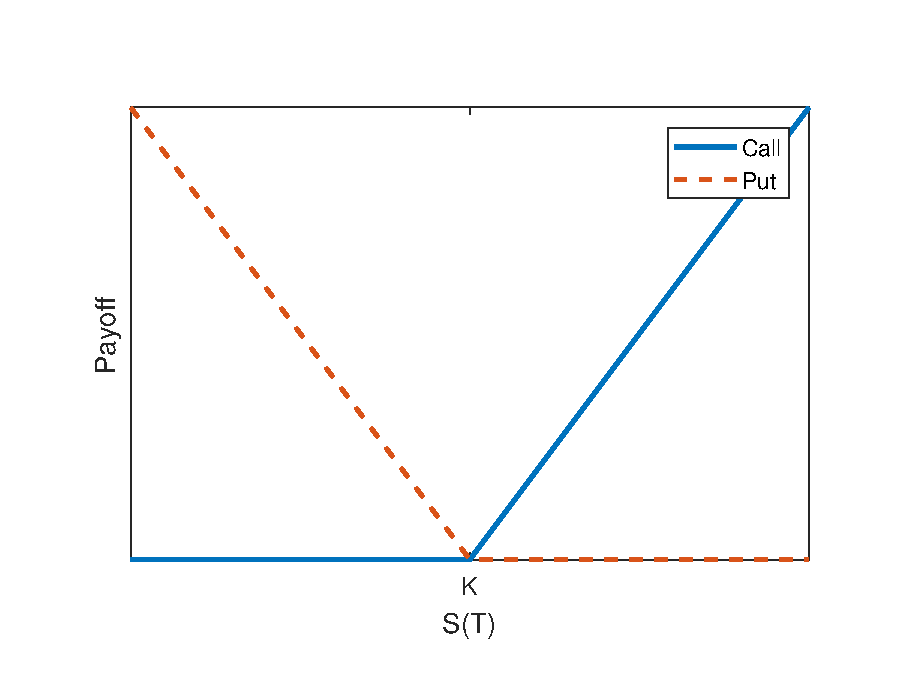
\includegraphics[width=.65\columnwidth]{Payoff.eps}
      \caption[Payoff functions of European call and put options]{Payoff functions of European \emph{call} and \emph{put options}.}\label{fig:Payoff}
    \end{figure}
    



\subsection{American Options}
\emph{American options} are more complex than European and thus harder to price. While European options dominate the OTC market, their American counterparts are the most traded type of option in exchanges~\citep{InvAmer}. Because of their great importance, many models have been developed to find the prices of these options~\citep{Longstaff}.

American options grant the right to buy/sell (call/put) the underlying asset at any point in time \emph{until the maturity date}. Following the logic used in the previous example to find the payoff functions of European calls and puts, we can deduce their American counterparts as
\begin{equation}
\begin{split}
&\text{Payoff}_{Amer,\ call}(K,t^*)=\max\left(S(t^*)-K,0\right);\\
&\text{Payoff}_{Amer,\ put}(K,t^*)=\max\left(K-S(t^*),0\right),
\end{split}
\end{equation}
\noindent where we now define $t^*$ (with $0\leq t^*\leq T$) as the exercise date.

It should be obvious that the price of American options will always be greater than or equal to the prices of equivalent European options. The reason behind this is the fact that with European contracts our exercising decision is restricted to a single day, whereas with American options we have that same day as well as several others to make this choice.


\subsection{Exotic Options}
While European and American options are, by far, the most traded types, \emph{Exotic options} should not be neglected. Not only does there exist a great number of Exotic option types, but these are also highly customizable, making this type of derivatives ideal for unconventional investment strategies. Due to their high complexity, these options are only traded in the OTC market, and not in exchanges~\citep{InvExotic}. We will explore one of the most common types of Exotic options - \emph{Barrier} options - though many others exist.


\subsubsection{Barrier Options}
A \emph{Barrier option} behaves similarly to a European option with the difference that it only becomes active (or becomes worthless) if the value of its underlying asset reaches a particular value, called the \emph{barrier level}, $B$, at any point in time until the option's maturity.

There are four main types of Barrier option:
\begin{itemize}
\item \emph{up-and-out}: the asset's price starts below the barrier (i.e. $S(0)<B$). If it increases past this threshold, the option becomes \emph{worthless};
\item \emph{down-and-out}: the asset's price starts above the barrier (i.e. $S(0)>B$). If it decreases past this threshold, the option becomes \emph{worthless};
\item \emph{up-and-in}: the asset's price starts below the barrier (i.e. $S(0)<B$). \emph{Only if} it increases past this threshold does the option become \emph{active};
\item \emph{down-and-in}: the asset's price starts above the barrier (i.e. $S(0)>B$). \emph{Only if} it decreases past this threshold does the option become \emph{active}.
\end{itemize}

Because all of the previously described Barrier option types are handled similarly, we can easily adapt the models from one type to another. Thus, for simplicity, we will henceforth assume that all Barrier options are of the up-and-in type.

We now deduce the payoff function of this type of Exotic contract. Using the up-and-in Barrier option type as an example, if the asset price, $S(t)$, remains below the barrier level $B$ throughout the whole option duration, even if at the maturity the asset's value is higher than the strike price, the option's payoff would nonetheless be zero. On the contrary, if this threshold was surpassed at any point during this period, the option's payoff would be similar to that of its European equivalent.
The payoff function of this type of option is therefore given by
\begin{equation}\label{barrier}
\begin{split}
&\text{Payoff}_{Barr,\ call}(K,T)=\begin{cases} 
      \max\left(S(T)-K,0\right), & \mathrm{if}\ \ \exists\,t<T\,:\,S(t)>B\\
      0, & \mathrm{otherwise}
   \end{cases};\\
&\text{Payoff}_{Barr,\ put}(K,T)=\begin{cases} 
      \max\left(K-S(T),0\right), & \mathrm{if}\ \ \exists\,t<T\,:\,S(t)>B\\
      0, & \mathrm{otherwise}
   \end{cases}.
\end{split}
\end{equation}


Before simulating Barrier options and studying their behavior, we can deduce the effect of the barrier level $B$ on the overall price of the option. For an up-and-in Barrier option, if the barrier level is too high, the price of the option will be very low. This is due to the fact that the likelihood of a stock price increasing enough to surpass such a high barrier level, activating the option, is very low. On the other hand, if the barrier level is very close to $S_0$, the probability of the stock price reaching this threshold is approximately $1$. Thus, the price of such an option would be very similar to that of its European equivalent.
With these two examples, we can conclude that the higher the barrier level, the lower the Barrier option price.

From eq.\eqref{barrier} we can furthermore conclude that the prices of Barrier options are always smaller than or equal to those of their equivalent European counterparts (i.e. with same strike and maturity). This should be straightforward, since the Barrier option becomes equal to its European counterpart only if the Barrier threshold is broken, and is worthless otherwise.




Though Exotic options are used by banks and investors everyday, we will mainly focus on European options: not only are these the most common type of option traded, as we mentioned before, but data is also readily available for many different maturities and strike prices, making European options ideal for model calibration and validation, which will be the main goal of this thesis.
Barrier options will nonetheless be implemented and studied, though no benchmark will be used to verify the models' validity in this case.


\section{Option Prices and Payoffs}
It is important to emphasize the difference between an option's payoff and its profit for investors. Because options grant the right to buy/sell some asset, no investors would exercise an option if this action was disadvantageous to them (i.e. negative payoff value, which is very unlikely to occur~\citep{Wilmott}). Thus, the payoff of an option is always positive (it can also, obviously, be zero). This might sound like an arbitrage possibility (i.e. the chance of making profit without risk), but in reality options have a price that investors have to pay in order to acquire them. This means that even if the option's payoff is positive, if this value is lower than the price an investor paid to buy the option, that investor will actually lose money. The profit of an option is thus the difference between its payoff and its price, which can be negative.
With this concept in mind, we can price options by setting their expected profit to be the same as a risk-neutral investment, (e.g. bank deposit). The price of an option can thus be deduced as it's expected future payoff, discounted back to the present
\begin{equation}\label{pricepayoff}
\text{Price}(K,t^*)=e^{-rt^*}\mathbb{E}\left[\text{Payoff}(K,t^*)\right],
\end{equation}
\noindent where $t^*$ denotes the time at which the option is exercised and $r$ corresponds to the risk-free interest rate, which we will approach in \autoref{section:Black-Scholes Formulae}.
In particular, with eqs.\eqref{callput} in mind, the price functions of European call and put options is clearly given by
\begin{equation}\label{callprice}
\begin{split}
&C(K,T)_{Euro}=e^{-rT}\mathbb{E}\left[\max\left(S(T)-K,0\right)\right]=e^{-rT}\mathbb{E}\left[\left(S(T)-K\right)\mathbbm{1}_{\left\{S(T)>K\right\}}\right];\\
&P(K,T)_{Euro}=e^{-rT}\mathbb{E}\left[\max\left(K-S(T),0\right)\right]=e^{-rT}\mathbb{E}\left[\left(K-S(T)\right)\mathbbm{1}_{\left\{S(T)<K\right\}}\right],
\end{split}
\end{equation}
\noindent with $C(K,T)$ and $P(K,T)$ being the values (i.e. prices) of European call and put options, respectively, and $\mathbb{E}[\cdot]$, $\mathbbm{1}_{\{\cdot\}}$ corresponding to the expected value and indicator functions, respectively.

When selling or buying options, investment banks add some premium to this zero-profit price, to account for the risk taken. Though this premium is important to define, it is besides the scope of this work and will not be considered here.

\subsection{Put-Call Parity}
One important aspect of option prices is known as \emph{put-call parity}. It can be easily shown that the prices of call options are inherently related to the prices of put options with the same strike prices and maturities. This relationship is given by
\begin{equation}
C(K,T)=S(0)-Ke^{-rT}+P(K,T),
\end{equation}
\noindent where $S(0)$ denotes the stock price at inception (i.e. when the option is bought).

Because of this duality, we can always easily obtain the prices of put options from the prices of call options with the same underlying asset, maturity and strike. For this reason, some of the results presented in later sections only apply to call options, though we can just as easily find their put option equivalent.
    
\section{Black-Scholes Formulae}
\label{section:Black-Scholes Formulae}
Due to their high importance, options have been studied in great detail in the past.
Probably the most important result in this field came from Fischer Black, Myron Scholes and Robert Merton, who developed a mathematical model to price European options - the famous Black-Scholes (BS) model~\citep{Scholes} - still in use in present days~\citep{Wilmott3}.

This model states that the price of an European (call or put) option follows the partial differential equation (PDE)

\begin{equation}\label{BS2}
\boxed{\pdv{V}{t}+\frac{1}{2}\sigma^2S^2\pdv{^2V}{S^2}+rS\pdv{V}{S}-rV=0,}
\end{equation}

\noindent where $V$ is the price of the option, $S$ is the price of the underlying (risky) asset, $r$ is the risk-free interest rate and $\sigma$ is the stock price volatility.
The underlying asset is commonly referred to as \emph{stock}, so these terms will be used interchangeably in the following sections.

\begin{proof}
Itô's Lemma can be applied to our option price $V$, which depends on the (stochastic) stock price $S$ and time $t$, so that we obtain
\begin{equation}\label{BSproof}
dV=\pdv{V}{t}dt+\pdv{V}{S}dS+\frac{1}{2}\pdv{^2V}{S^2} (dS)^2.
\end{equation}

We now assume that the stock price $S$ follows a geometric Brownian Motion,
\begin{equation}\label{BSproofGBM}
dS(t)=rS(t)dt+\sigma S(t)dW(t),
\end{equation}
\noindent where $\{W(t),\ t>0\}$ is a Brownian motion process.

It can be shown that $(dW)^2=dt$, $(dt)^2=0$ and $(dt).(dW)=0$. With these properties in mind, we can substitute eq.\eqref{BSproofGBM} into eq.\eqref{BSproof}, giving
\begin{equation}
\begin{split}
dV=&\pdv{V}{t}dt+\pdv{V}{S}\left(rSdt+\sigma SdW\right)+\frac{1}{2}\left(rSdt+\sigma SdW\right)^2\pdv{^2V}{S^2}\\
=&\left(rS\pdv{V}{S}+\pdv{V}{t}+\frac{1}{2}\sigma^2S^2\pdv{^2V}{S^2}\right)dt+\sigma S\pdv{V}{S}dW.
\end{split}
\end{equation}


We now construct a portfolio where we sell \emph{one} option and buy an amount $\partial V/\partial S$ of stocks. The value of such a portfolio would be
\begin{equation}\label{pi}
\Pi=-V+\pdv{V}{S}S.
\end{equation}

From this equation we can easily derive the change of the portfolio's value, $d\Pi$, in the time interval $dt$ as
\begin{equation}\label{dpi}
\begin{split}
d\Pi&=-dV+\pdv{V}{S}dS\\
&=\left(\pdv{V}{t}+\frac{1}{2}\sigma^2S^2\pdv{^2V}{S^2}\right)dt.
\end{split}
\end{equation}

Because the portfolio's value doesn't change with the Brownian motion $\{W(t),\ t>0\}$, it follows that it must be \emph{riskless}.
To avoid any arbitrage possibilities (i.e. making profit without risk, which is very unlikely to happen), the value of this portfolio must be the same as any risk-free asset. The value of a portfolio with such an asset would change with time as
\begin{equation}\label{dpi2}
d\Pi=r\Pi dt.
\end{equation}

Substituting eqs.\eqref{pi} and\eqref{dpi} into eq.\eqref{dpi2} gives
\begin{equation}
\pdv{V}{t}+\frac{1}{2}\sigma^2S^2\pdv{^2V}{S^2}+rS\pdv{V}{S}-rV=0.
\end{equation}

\end{proof}


The risk-free interest rate, $r$, is the interest an investor would receive from any risk-free investment (e.g. treasury bills). No investor should ever invest in risky products whose expected return is lower than this interest (e.g. the lottery), since there's the alternative of obtaining a higher (expected) payoff without the disadvantage of taking risks. In general, this rate changes slightly with time and is unknown. Black \textit{et al.}, in their original model (eq.\eqref{BS2}), assumed that this rate is a known function of time. Some authors have suggested solutions to deal with this shortcoming, providing stochastic models to replicate the behavior of interest rates~\citep{HJM}, but because option prices do not significantly depend on this value~\citep{Wilmott3}, in the remainder of this thesis we shall set this rate to some constant.

As for the stock price volatility, $\sigma$, since we will explore it to great extent in \autoref{chapter:volatility}, suffice it to say for now that it is a measure of the future stock price movement's uncertainty.

Some companies decide to grant their shareholders a part of the profits generated, known as \emph{dividends}. This action decreases the company's total assets, which decreases the value of stocks, changing option prices. Because this occurrence is based on human behavior, it is extremely hard to model. Furthermore, Black \textit{et al.} assumed in their models that no dividends were paid throughout the option's duration. For both these reasons, we will set dividend payment to zero in all our models.


One other important assumption of the BS model is that stock prices follow a stochastic process, known as Geometric Brownian Motion, defined as
\begin{equation}\label{GBM}
dS(t)=rS(t)dt+\sigma S(t)dW(t),
\end{equation}
\noindent with $\{W(t),\ t>0\}$ defining a one-dimensional Brownian motion and where we define $S_0=S(0)$ as the stock price at time $t=0$. An example of such processes is represented in \autoref{fig:GBM}.

Many other diffusion processes exist, and this choice made by Black \textit{et al.} might seem a bit arbitrary, but there is actually a reason behind it. Changes in the stock price are geometric and not arithmetic. If an asset of price $1000\SI{}{\EUR}$ changed by $9\SI{}{\EUR}$, we would barely take notice. If another asset of price $10\SI{}{\EUR}$ changed by $9\SI{}{\EUR}$, the drop would be quite surprising, even though the change was the same in both assets. This seems to indicate that changes in the stock price depend on the stock price itself and justifies the choice made by Black \textit{et al.} to model stock prices using a Geometric Brownian Motion process.
\begin{figure}[!htb]
    \centering
      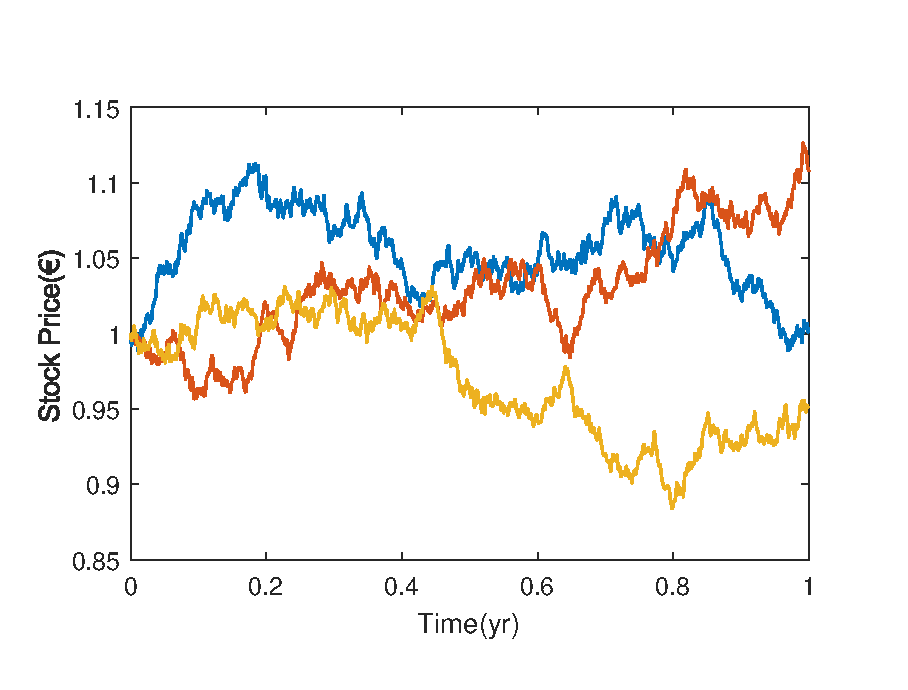
\includegraphics[width=.65\columnwidth]{GBM.eps}
      \caption[Example of Geometric Brownian Motion processes]{Example of three Geometric Brownian Motion processes with maturity $T=1\SI{}{\year}$, interest rate $r=0.01\SI{}{\per\year}$, volatility $\sigma=0.1\SI{}{\year\tothe{-1/2}}$ and initial stock price $S_0=1\SI{}{\EUR}$.}\label{fig:GBM}
    \end{figure}

With this result, pricing options is fairly straightforward - we simply need to solve the PDE in eq.\eqref{BS2} as we would for the diffusion equation's initial value problem~\citep{Dilao}.
The results published originally by Black \textit{et al.} state that call and put options can be valued as
\begin{subequations}\label{callputBS}
\begin{empheq}[box=\widefbox]{align}
&C=N(d_1)S_0-N(d_2)Ke^{-rT};\\
&P=-N(-d_1)S_0+N(-d_2)Ke^{-rT},
\end{empheq}
\end{subequations}
\noindent where $N(\cdot)$ is the cumulative distribution function of the standard normal distribution and where $d_1$, $d_2$ are given by
\begin{subequations}\label{d1d2}
\begin{empheq}[box=\widefbox]{align}
&d_1=\frac{1}{\sigma\sqrt{T}}\left[\log\left(\frac{S_0}{K}\right)+\left(r+\frac{\sigma^2}{2}\right)T\right];\\
&d_2=d_1-\sigma\sqrt{T}.
\end{empheq}
\end{subequations}

This is a very important result that can be used to precisely price European options, so long as all the parameters are exactly known and remain constant throughout the option's duration. Both assumptions are never true for any real market option, though.

In \autoref{fig:Inception} we represent the values of call and put options at both the inception (i.e. when the option is bought) and at maturity. Notice how at maturity the value functions tend to the payoff functions, shown in \autoref{fig:Payoff} (take into account that the x-axis in \autoref{fig:Payoff} represents $S(T)$ and in \autoref{fig:Inception} we have $K/S_0$, so they are opposite).
\begin{figure}[!htb]
    \centering
      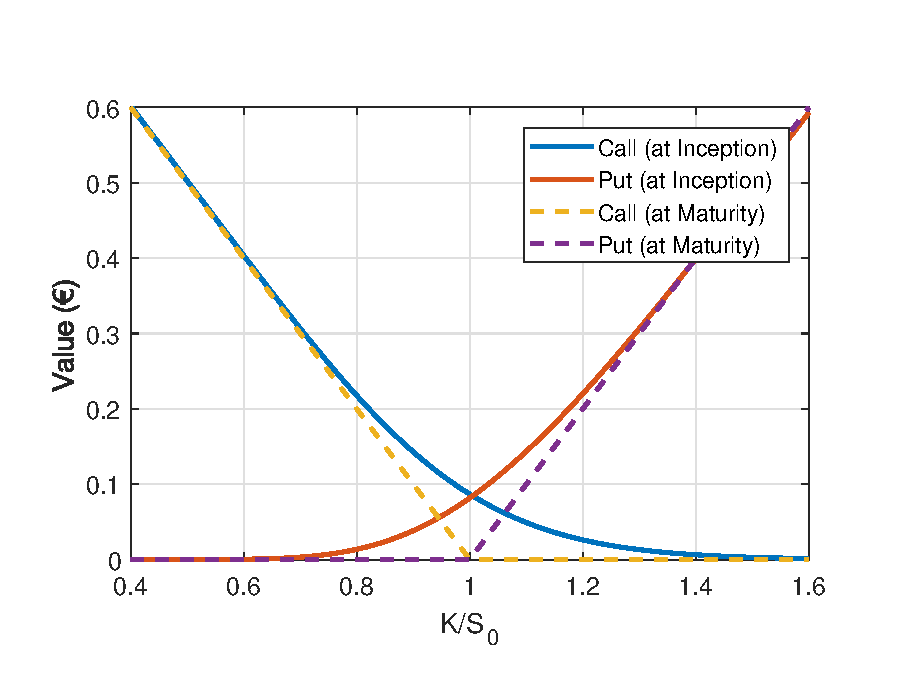
\includegraphics[width=.65\columnwidth]{Inception.eps}
      \caption[Call and Put option values at inception and maturity]{Call and Put option values at inception and maturity with $T=0.5\SI{}{\year}$, interest rate $r=0.01\SI{}{\per\year}$, volatility $\sigma=0.3\SI{}{\year\tothe{-1/2}}$ and initial stock price $S_0=1\SI{}{\EUR}$.}\label{fig:Inception}
    \end{figure}


\iffalse
\subsubsection{Barrier Options}
As we did for European call and put options, we can equally derive the theoretical prices of Barrier options, changing the boundary condition to incorporate the barrier level~\citep{taleb}. The resulting \emph{up-and-in call} Barrier option price is given by
\begin{equation}\label{barr1}
C_{Barr}^*=S_0\left(N(d_3)+b\left(N(d_4)-N(d_5)\right)\right)-Ke^{-rT}\left(N(d_6)+a\left(N(d_7)-N(d_8)\right)\right),
\end{equation}
\noindent where we define the variables $a$, $b$ and $d_3$ through $d_8$ as
\begin{equation}
a=\left(\frac{B}{S_0}\right)^{-1+\frac{2r}{\sigma^2}},
\end{equation}
\begin{equation}
b=\left(\frac{B}{S_0}\right)^{1+\frac{2r}{\sigma^2}},
\end{equation}
\begin{equation}
d_3=\frac{1}{\sigma\sqrt{T}}\left[\log\left(\frac{S_0}{B}\right)+\left(r+\frac{\sigma^2}{2}\right)T\right],
\end{equation}
\begin{equation}
d_4=\frac{1}{\sigma\sqrt{T}}\left[\log\left(\frac{S_0}{B}\right)-\left(r+\frac{\sigma^2}{2}\right)T\right],
\end{equation}
\begin{equation}
d_5=\frac{1}{\sigma\sqrt{T}}\left[\log\left(\frac{S_0K}{B^2}\right)-\left(r+\frac{\sigma^2}{2}\right)T\right],
\end{equation}
\begin{equation}
d_6=\frac{1}{\sigma\sqrt{T}}\left[\log\left(\frac{S_0}{B}\right)+\left(r-\frac{\sigma^2}{2}\right)T\right],
\end{equation}
\begin{equation}
d_7=\frac{1}{\sigma\sqrt{T}}\left[\log\left(\frac{S_0}{B}\right)-\left(r-\frac{\sigma^2}{2}\right)T\right],
\end{equation}
\begin{equation}
d_8=\frac{1}{\sigma\sqrt{T}}\left[\log\left(\frac{S_0K}{B^2}\right)-\left(r-\frac{\sigma^2}{2}\right)T\right],
\end{equation}
\noindent where $B$ defines the barrier level, at which the option becomes activated.

We should note that the formula in eq.\eqref{barr1} only holds for Barrier options with barrier levels greater than the strike price (i.e. $B>K$).
For the cases where this condition is not met, the Barrier option price should be equal to that of its European counterpart. To see this, we note that a (up-and-in) Barrier option only has value if, at the maturity, the stock price is greater than the strike \emph{and} the barrier was broken until then. If the barrier level is lower than the strike, the option can't reach the strike price without breaking the barrier, which means that the second constraint is pointless. Thus, in this case, the Barrier option price is equal to its European counterpart.
The real price of an up-and-in call Barrier option is therefore
\begin{equation}\label{barr2}
C_{Barr}=\begin{cases} 
      C_{Barr}^*, & \mathrm{if}\ \ \ B>K\\
      C_{Euro}, & \mathrm{otherwise}
   \end{cases}
\end{equation}
\noindent where $C_{Barr}^*$ is given by eq.\eqref{barr1} and $C_{Euro}$ is the equivalent European option price.

\fi
